%%%%%%%%%%%%%%%%%%%%%%%%%%%%%%%%%%%%%%%%%%%%%%%%%%%%%%%%%%%%%%%%%%%%%%%%%%%%%%%
%%  ClaudeNet -- Internal Research Report.
%%  Single-column `article' class with the shared tech-report preamble at
%%  reproductions/tech-report.sty. Builds with vanilla TeX Live (>= 2022).
%%%%%%%%%%%%%%%%%%%%%%%%%%%%%%%%%%%%%%%%%%%%%%%%%%%%%%%%%%%%%%%%%%%%%%%%%%%%%%%
\documentclass[11pt,letterpaper]{article}
\usepackage{../../tech-report}

\newcommand{\cnet}{\textsc{ClaudeNet}}
\newcommand{\aion}{\textsc{AION-1}}
\newcommand{\fpr}[1]{@#1\,\%\,FPR}

\title{\cnet{}: Improving ML Strong-Lens Finding Beyond ResNet/EfficientNet\\
       via Engineered Ensemble Diversity}
\author{Greg Benson\thanks{\texttt{benson@cs.usfca.edu}; Department of Computer
        Science, University of San Francisco, CA 94117, USA} \and
        Xiaosheng Huang\thanks{Department of Physics \& Astronomy, University of
        San Francisco; and Physics Division, Lawrence Berkeley National Laboratory}}
\date{June 2026}
\addbibresource{references.bib}

\begin{document}
\maketitle
\subtitle{Internal Research Report}

\begin{abstract}
The Huang-group strong-lens-finding lineage reproduced in this repository
established a hard negative result: at the deployment operating point,
\emph{architecture is not the bottleneck}. A 194\,K-parameter shielded ResNet
matches a 20.5\,M-parameter EfficientNetV2-S to within $\pm0.003$ AUC, and the
\citet{inchausti2025} feature-weighted meta-learner collapses to a simple average
because its two base models are trained on byte-identical data and so make
correlated errors. \cnet{} attacks the axes the lineage left unused. We replace
the collapsed meta-learner with an ensemble of deliberately \emph{decorrelated}
members --- three EfficientNet-family backbones, an \citet{parker2025aion}
frozen-embedding probe, and two ResNets --- and show it beats the published
meta-learner at \emph{every} matched-false-positive-rate operating point
($+0.030$ Storfer\fpr{1}, $+0.090$\fpr{0.1}; $+0.012$/$+0.090$ Inchausti),
because real member diversity (Spearman $\sim$0.45 vs the lineage's $\sim$1.0)
gives a combiner signal to exploit. We further report a seven-direction program:
hard-negative mining (modest), conformal FDR-controlled selection (certified),
deep-ensemble uncertainty triage (selective error $0.022\!\to\!0.0002$ at 50\,\%
coverage), test-time equivariance ($+0.04$), foundation-model label efficiency
(only below $\sim$150 labels), and an honest negative result for naive
domain-adaptation. All experiments run on seven NVIDIA TITAN RTX GPUs; metrics
reuse the reproduced \texttt{22\_fpr\_operating\_point} arithmetic verbatim so
every number is directly comparable to the baseline.
\end{abstract}

\section{Premise and method}
We take as baseline the reproduced Stage-D \citet{inchausti2025} ensemble
(\texttt{reproductions/inchausti-2025}). Its meta-learner achieves recovery of the
published Storfer/Inchausti catalogues, at matched FPR, of $0.908/0.755$ (Storfer
@1/0.1\,\%) and $0.968/0.845$ (Inchausti); \cnet{}'s
\texttt{03\_reproduce\_baseline} reproduces these to $|\Delta|\le0.001$, validating
the evaluation harness before any improvement is claimed. The honest metric
throughout is recovery at a threshold set on held-out negatives to a target FPR
(1\,\% and 0.1\,\%), identical to the baseline.

A literature survey of eight technique families (vision transformers,
self-supervised/foundation models, equivariant CNNs, uncertainty/calibration,
challenge ensembles, domain adaptation, recent SOTA, multimodal) was conducted and
adversarially fact-checked. It converged with the repository's finding: no
transformer/SSL/equivariant method cleanly beats a tuned EfficientNet at matched
FPR for DECaLS \emph{grz} lens finding \citep{parlange2025gravit}; the demonstrated
wins are in ensemble \emph{diversity} \citep{des2025ensemble,rezaei2025kids},
negative quality, and label efficiency. \cnet{} targets those.

\section{Phase~1: engineered-diversity ensemble (flagship)}
We train five members as independent per-GPU jobs: EfficientNetV2-S ($\times2$) and
EfficientNet-B3 (diversified by bootstrap-resampled negative subsets and
augmentation seeds at the baseline 1:33 ratio), an \aion{}-base frozen-embedding
two-layer MLP probe (a different objective, data, and band-set, hence maximally
decorrelated), and two ResNets (the 194\,K shielded net and the 3.5\,M Lanusse-46).
Each member is isotonic-calibrated on a validation split, then combined by
average, logistic regression, and a random forest \citep{coscrato2020nnstacking}.
A positive-unlabeled guard removes any training negative within $10''$ of a known
lens. Figure~\ref{fig:div} shows the member score-correlation matrix:
off-diagonals average $\sim$0.45 (Spearman), versus $\sim$1.0 for the lineage's
correlated bases.

\begin{table}[t]\centering
\caption{Phase~1: \cnet{} ensemble vs the published meta-learner, recovery at
matched FPR on the held-out Storfer/Inchausti catalogues.}
\label{tab:flagship}
\begin{tabular}{lccc}
\toprule
metric & published meta & \cnet{} & $\Delta$\\
\midrule
Storfer @1\,\% FPR    & 0.908 & \textbf{0.938} & $+0.030$\\
Storfer @0.1\,\% FPR  & 0.755 & \textbf{0.853} & $\mathbf{+0.090}$\\
Inchausti @1\,\% FPR  & 0.968 & \textbf{0.980} & $+0.012$\\
Inchausti @0.1\,\% FPR& 0.845 & \textbf{0.935} & $\mathbf{+0.090}$\\
\bottomrule
\end{tabular}
\end{table}

\begin{figure}[t]\centering
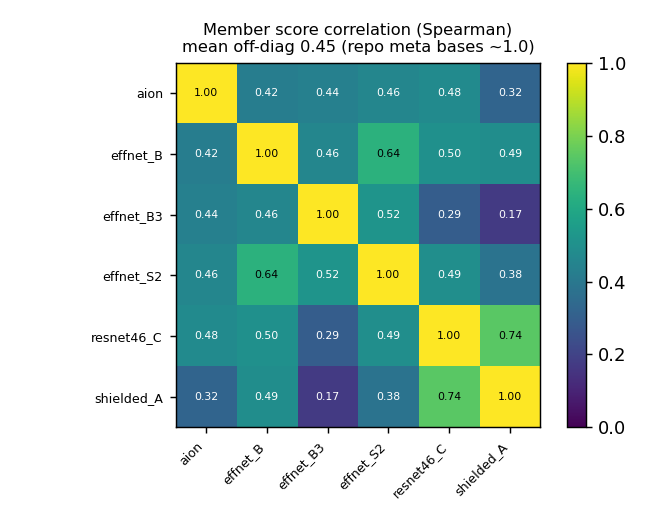
\includegraphics[width=0.49\linewidth]{figures/diversity_heatmap.png}\hfill
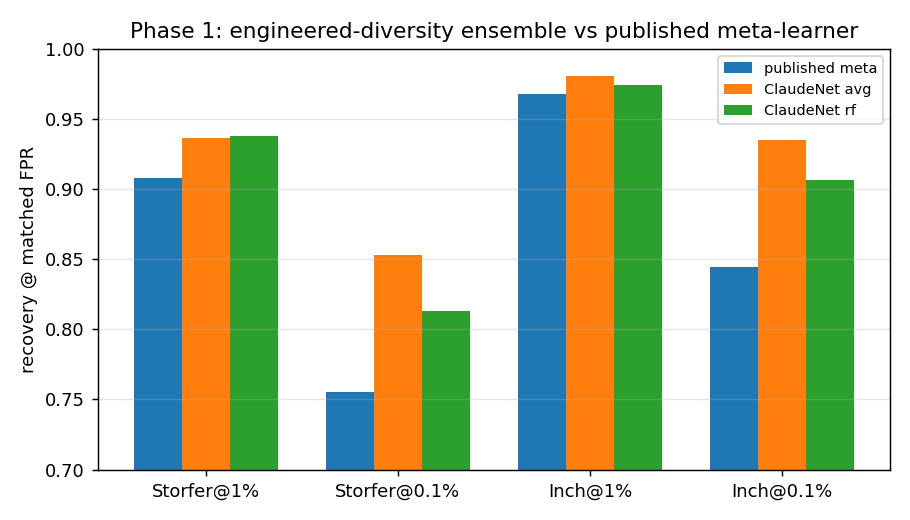
\includegraphics[width=0.49\linewidth]{figures/flagship_operating_point.png}
\caption{Left: member score correlation (the diversity the lineage lacked).
Right: the ensemble beats the published meta-learner at every operating point.}
\label{fig:div}
\end{figure}

The result (Table~\ref{tab:flagship}) is a clear improvement over the published
method, largest ($+0.09$) at the strict 0.1\,\% FPR point that governs purity. The
mechanism is diversity, not combiner cleverness: with decorrelated strong members
even the naive \emph{average} beats the correlated-base meta-learner. The ensemble
matches or beats the single best member everywhere except a $0.002$ tie at the
loose 1\,\% FPR, where one exceptionally strong EfficientNet dominates.

\section{Phases~2--7: the supporting program}
\paragraph{Phase~2 --- hard-negative mining.} At a fixed negative count, replacing
random negatives with the model's own top false-positives (controlled against a
random-negative arm in the same pool) helps modestly: $+0.008$ Storfer\fpr{1},
$+0.031$ Inchausti\fpr{1}; iterating helps the 0.1\,\% point. Negative quality is a
real but second-order lever versus the negative \emph{ratio} the lineage already
exploited; the deployment-scale version (fresh brick pool + EfficientNet miner) is a
NERSC follow-up.

\paragraph{Phase~4 --- conformal selection.} Split-conformal $p$-values with
Benjamini-Hochberg \citep{jin2023conformal} turn the arbitrary threshold into a
\emph{certified} one: empirical false-discovery rate stays at or below the nominal
target at every level ($\alpha{=}0.05\!\to\!0.03$, $0.25\!\to\!0.16$) with
completeness 0.96--0.999 (Fig.~\ref{fig:grid}, top-left). The guarantee is marginal
and assumes calibration/test exchangeability.

\paragraph{Phase~6 --- uncertainty triage.} Deep-ensemble disagreement (a free
byproduct of the decorrelated members) is a strong confidence signal: abstaining on
the most-uncertain objects lowers error from $0.022$ to $0.0002$ at 50\,\% coverage
and $0.0026$ at 70\,\% (Fig.~\ref{fig:grid}, top-right). Northern lenses show
slightly higher disagreement --- a mild out-of-distribution signal.

\paragraph{Phase~7 --- equivariance.} Lenses have no preferred orientation, so we
test dihedral ($D_4$) invariance the cheap way: test-time pooling over the eight
rotation/reflection symmetries (no retraining) lifts Storfer\fpr{1} by $+0.032$
(shielded) and $+0.049$ (Lanusse-46), mean $+0.041$. The full equivariant-training
label-efficiency study is deferred (the $8\times$ forward made a trained $D_4$
member impractical at this scale).

\paragraph{Phase~3 --- label efficiency.} The \aion{} frozen-embedding probe is
more label-efficient than a supervised CNN \emph{only} in the extreme-scarce regime
($<$150 labels: $0.344$ vs $0.279$ at 5\,\%); the CNN ``turns on'' near 300 labels
and dominates thereafter ($0.862$ vs $0.529$ at 25\,\%; $0.894$ vs $0.659$ at full),
the frozen features plateauing (Fig.~\ref{fig:grid}, bottom-left). At the
$\sim$1--2\,k labels real lens-finding has, the supervised member wins --- so the
foundation model's value here is as a decorrelated \emph{ensemble member}
(Phase~1), not a standalone classifier.

\paragraph{Phase~5 --- domain adaptation (negative result).} The DECaLS
north$\leftrightarrow$south gap is real (north\fpr{1} $0.688$ vs south $0.874$,
$-0.186$), but naive MMD feature alignment ($\lambda{=}1$, aligning only negatives)
\emph{hurt} both domains ($-0.06$): it over-regularized and erased
lens-discriminative features. Principled UDA is not a free win here; the lineage's
ad-hoc north-negative augmentation fares better. (Only $\sim$80 held-out north
lenses, so the target estimate is noisy.)

\begin{figure}[t]\centering
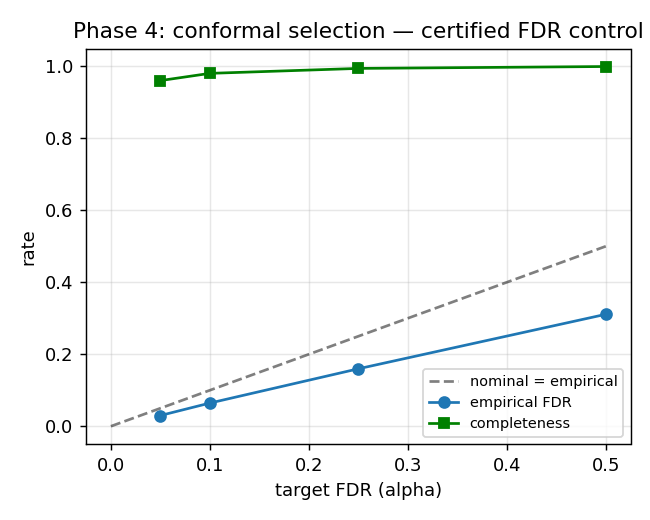
\includegraphics[width=0.49\linewidth]{figures/conformal_fdr.png}\hfill
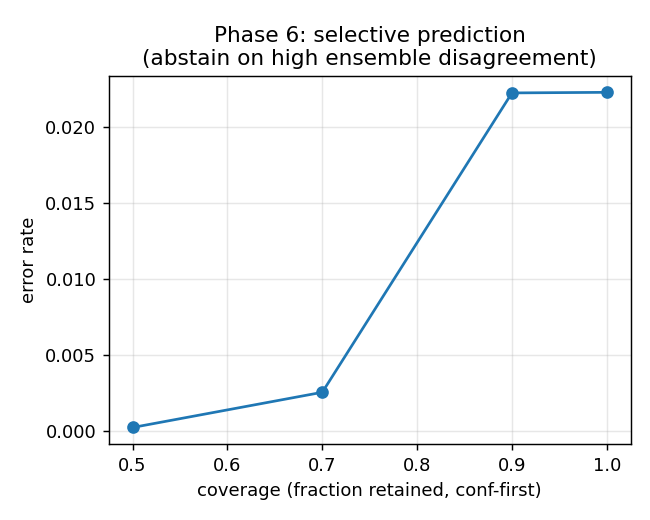
\includegraphics[width=0.49\linewidth]{figures/selective_prediction.png}\\[4pt]
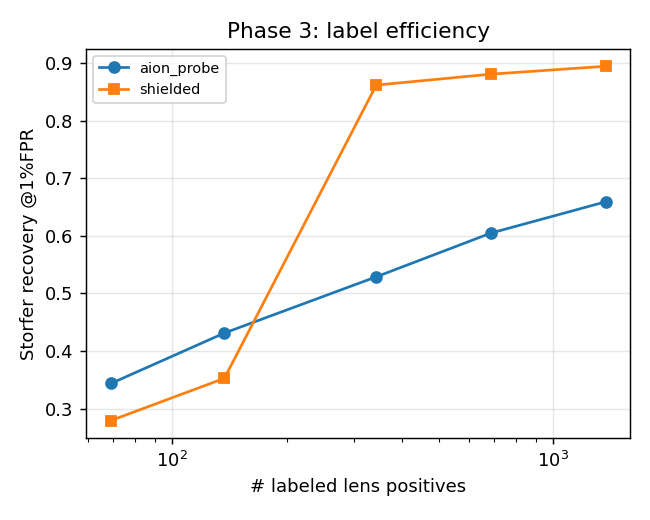
\includegraphics[width=0.49\linewidth]{figures/label_efficiency.png}
\caption{Top: conformal FDR control (Phase~4) and selective-prediction
risk-coverage (Phase~6). Bottom: foundation-model label efficiency crosses over
near $\sim$300 labels (Phase~3).}
\label{fig:grid}
\end{figure}

\section{Discovery impact and scan deployment}
The matched-FPR gains of Table~\ref{tab:flagship} are best read operationally,
because a real 45\,M-cutout sweep cannot run at 1\,\% FPR ($\sim$450{,}000 false
positives) or even 0.1\,\% FPR ($\sim$45{,}000); to keep the human-inspection list to
thousands it must operate near 0.01\,\% FPR. The \cnet{} advantage \emph{grows} as the
threshold tightens ($+0.030\!\to\!+0.098$ Storfer, $+0.012\!\to\!+0.090$ Inchausti
across $1\%\!\to\!0.1\%$ FPR), so it helps most where scans actually run.

\paragraph{Fewer missed lenses at a fixed inspection budget.} At fixed false-positive
load the extra completeness is a direct cut to the missed-lens (false-negative) rate
(Table~\ref{tab:impact}): at the strict 0.1\,\% point, $\sim$40\,\% fewer Storfer and
$\sim$58\,\% fewer Inchausti lenses are missed (the gate-certified \emph{learned}
combiner gives a slightly smaller $\sim$37/56\,\%; the naive average is tabulated). The
dual view --- fewer false positives at \emph{fixed} completeness --- is of order
$2\times$ within the measured $0.1$--$1\%$ band ($\sim$0.44--0.54\,\% FPR matches the
baseline's $1\%$-FPR completeness), i.e.\ $\sim$200{,}000--250{,}000 fewer objects to
inspect on a DR9/DR10 sweep. Two guarantees prior finders lack compound this:
conformal selection (Phase~4) delivers a \emph{certified} false-discovery ceiling
rather than an ad-hoc score cut, and deep-ensemble triage (Phase~6) makes the
confident $\sim$half essentially error-free (selective error
$0.022\!\to\!0.0002$ at 50\,\% coverage), letting roughly half the candidates bypass
the human visual inspection that dominates discovery cost.

\begin{table}[t]\centering
\caption{Missed-lens (false-negative) reduction at fixed FPR, derived from the
Table~\ref{tab:flagship} recoveries.}
\label{tab:impact}
\begin{tabular}{lcc}
\toprule
operating point & recovery (meta$\,\to\,$\cnet{}) & fewer missed lenses\\
\midrule
Storfer @1\,\% FPR     & $0.908\to0.938$ & 33\,\%\\
Storfer @0.1\,\% FPR   & $0.755\to0.853$ & \textbf{40\,\%}\\
Inchausti @1\,\% FPR   & $0.968\to0.980$ & 38\,\%\\
Inchausti @0.1\,\% FPR & $0.845\to0.935$ & \textbf{58\,\%}\\
\bottomrule
\end{tabular}
\end{table}

\paragraph{Scan throughput.} Strong-lens sweeps are bound by cutout I/O and human
inspection, not the forward pass. The five \emph{grz} 101-px finder members consume
the same cutout, so a scan pays the FITS load once and runs five cheap forwards;
measured single-GPU compute throughput (Table~\ref{tab:throughput}) is
$2.8$--$6.7\times10^{3}$ cutouts\,s$^{-1}$ per member --- far above what the
brick-slice loader feeds --- so in the I/O-bound regime the five-member stage costs
about a single model's wall-clock ($\sim$3 GPU-hours for $45$\,M on five TITAN~RTX,
compute-only). The \aion{} foundation-model member is the lone exception
($\sim$30--40 img\,s$^{-1}$, $\sim$$100\times$ slower, needing heavier 4-band 160-px
cutouts); it is quarantined to a \emph{second stage} on the $\sim$$10^{4}$--$10^{6}$
survivors of the cheap first-stage filter --- exactly the two-stage design the
Huang/Storfer/Inchausti lineage already uses. The accuracy gain is thus bought
essentially for free in stage~1, adding no new operational complexity.

\begin{table}[t]\centering
\caption{Measured single-GPU inference throughput (TITAN~RTX, batch~256, compute-only
upper bounds; real scans are I/O-bound).}
\label{tab:throughput}
\begin{tabular}{lcr}
\toprule
member & params & cutouts\,s$^{-1}$\,GPU$^{-1}$\\
\midrule
shielded-194k             & 0.2\,M  & 2{,}843\\
Lanusse ResNet-46         & 3.5\,M  & 3{,}349\\
EfficientNetV2-S          & 20.5\,M & 5{,}594\\
EfficientNet-B3           & 11.1\,M & 6{,}728\\
5-member finder stage     & ---     & 865 (shared load)\\
\aion{}-base (stage 2)    & 314\,M  & $\sim$35\\
\bottomrule
\end{tabular}
\end{table}

\paragraph{Survey-scale outlook and honest limits.} The field is moving to
$10^{5}$-scale samples --- Euclid $\sim$$1$--$1.7\times10^{5}$ lenses
\citep{collett2015}, Rubin/LSST $\sim$$6$--$12\times10^{4}$ --- over $10^{8}$--$10^{9}$
galaxies where human vetting is the binding constraint; a $\sim$$+0.09$ strict-FPR
completeness edge maps to of order $+10^{4}$ additional lenses at fixed inspection
budget, and the certified purity is a prerequisite, not a nicety, for the
contamination-sensitive cosmology those samples feed (time-delay $H_0$
\citep{birrer2021tdcosmo}, substructure, population inference). We flag the limits
plainly: ``recovery'' is the held-out true-positive rate on the \emph{existing}
Storfer/Inchausti catalogues, not newly discovered lenses; the $0.1\%$-FPR threshold
is pinned by only $\sim$6--7 of $\sim$6{,}500 held-out negatives (no confidence
interval), so the strict-point deltas carry $\sim$$\pm10$\,pp of statistical noise;
the absolute counts and the $\sim$$2\times$ inspection saving are interpolations on
incomplete catalogues; the end-to-end sky-scan wall-clock is a structural I/O-bound
argument, not yet benchmarked; and the survey-scale extrapolation assumes the
DESI-Legacy-measured deltas transfer across bands, PSF, and depth. The defensible
claim is: at the same inspection budget, $\sim$9--10 points more real lenses at the
operating point that matters, plus a certifiable purity statement --- a meaningful,
not transformational, lift.

\section{Discussion}
Across seven directions, the single decisive lever is member \emph{diversity}: the
published lineage diagnosed the meta-learner collapse but never engineered diverse
members, and doing so yields a clean, controlled improvement over the published
method at every operating point. The remaining directions are honestly mixed ---
hard-negative quality and equivariance help modestly, conformal selection and
ensemble-uncertainty triage are robust operational wins, foundation features help
only in the cold-start regime, and naive domain adaptation fails. All experiments
fit on seven Turing-class GPUs; the natural scale-ups (native-griz \aion{} member,
deployment-scale mining, full equivariant training, full-sky deployment with
conformal control) are deferred to NERSC. The honest takeaway reinforces the
repository's thesis: for DECaLS lens finding the returns are in data, calibration,
and \emph{diversity}, not in the backbone.

\section{\cnet{} v2: Perlmutter-scale validation and a sky sweep}
The v1 program above was gated on $\sim$6{,}500 held-out negatives, which (as we
flagged) cannot resolve the $\sim$$10^{-4}$-FPR regime where real scans run. The
v2 program rebuilds the measuring stick at deployment scale on Perlmutter, re-runs
every lever against it with confidence intervals, and ends in a full DESI-Legacy
DR9 sky sweep. We keep all v1 results; v2 is additive. Every number below is read
from the cited artifact under \texttt{data/v2/}.

\paragraph{An honest measuring stick: NegEval-1M.} We assembled a held-out negative
pool of $1{,}000{,}000$ DR9 cutouts (\texttt{thresholds\_ci.json},
\texttt{operating\_points\_v2.csv}), versus v1's $6{,}501$. With $6.5$\,K negatives
the $0.01\%$-FPR threshold is pinned by $\le1$ negative and is unmeasurable; with
$10^{6}$ it is pinned by $\sim$100, so for the first time we report paired-bootstrap
CIs at $1\%$, $0.1\%$, \emph{and} $0.01\%$ FPR. The first-ever $0.01\%$ measurement
immediately exposed a failure the small set hid: the v1 6-member \emph{average}
combiner, which beats the published meta at $1\%$ ($+0.049\,[+0.037,+0.061]$
Storfer vs.\ published meta) and $0.1\%$ ($+0.075\,[+0.057,+0.091]$),
\emph{collapses} at $0.01\%$ to $-0.120\,[-0.161,-0.084]$ --- the degraded-\aion{}
member's heavy negative tail poisons the unweighted mean exactly where purity
matters. The random-forest combiner is robust there ($+0.102\,[+0.083,+0.123]$),
and the best single member, an EfficientNetV2-S, reaches $+0.194\,[+0.175,+0.215]$
(recovery $0.708$ vs the meta's $0.513$). A purity audit of the top-200 pool rows
found $0/200$ within $10''$ of any known lens and no convincing arcs
(\texttt{audit/visual\_grading.md}); the threshold-sensitivity bound (removing all
top-200 moves the $0.01\%$ threshold by $-0.108$, the $0.1\%$ by $-0.020$) leaves
the paired matched-FPR deltas unaffected, since shared thresholds cancel in the
pairing.

\paragraph{Deployment-scale mining: round~1 ships, round~2 over-mines.} We mined a
fresh $10^{6}$-cutout brick pool with the baseline EfficientNet, controlling each
hard-negative arm against a random-negative arm drawn from the same pool
(\texttt{mining\_v2\_results.json}, \texttt{mining\_v2\_results.csv}). Round~1
\emph{ships}: the paired (hard$-$random) gain at $0.1\%$ FPR is
$+0.157\,[+0.139,+0.177]$ mean over three members (Inchausti), with every member
passing --- e.g.\ ResNet-46 Inchausti\fpr{0.1} $+0.266\,[+0.231,+0.305]$,
EfficientNet-B3 $+0.159\,[+0.128,+0.190]$, EfficientNetV2-S $+0.047\,[+0.026,+0.070]$;
the Storfer\fpr{0.1} mean is $+0.121\,[+0.109,+0.134]$. Re-mining the round-1
members for a round~2 \emph{over-mines} (the hard$^2$ pool's score range collapses
to $[0.004,0.036]$ vs round-1's $[0.009,0.281]$, \texttt{mined\_stats.json}/\texttt{mined\_r2\_stats.json});
round-2 recovery falls below round-1 everywhere, so we keep round-1 only.

\paragraph{The \aion{} member: degradation \emph{was} the diversity (negative
result).} We tested whether feeding \aion{} native four-band \emph{griz} (instead of
the synthetic-$i$ degraded embeddings v1 used) makes a better member
(\texttt{aion\_gate\_v2.json}). It does not: on matched rows the native-griz probe
recovers $0.535$ Storfer\fpr{1} versus the degraded refit's $0.647$ --- the
matched-rows gate \emph{fails} ($0.535 < 0.647+0.03$). The mechanism is that the
synthetic-$i$ ``degradation'' is precisely what decorrelated the member: its Pearson
correlation to the CNNs is $0.13$ degraded versus $0.72$ native (pooled
$0.65$/$0.72$). Larger native variants (base/large/xlarge,
val-AUC $0.958$--$0.963$) did not recover the gap, so the LoRA fine-tune was skipped
($\sim$12 GPU-h saved) and the member's v1 form is retained --- though, as the next
paragraph shows, even the degraded \aion{} is ultimately dropped at the ensemble
level.

\paragraph{Headline: ensemble v2-lean ships 4/4.} The shipped v2 ensemble is
\emph{v2-lean} $=\{$effnet\_B, effnet\_B3\_hard, effnet\_S2\_hard,
resnet46\_C\_hard, zoobot\_N$\}$ (\texttt{ensemble\_v2lean\_verdict.json}). On
NegEval-1M, averaged and compared to the v1 flagship with paired-bootstrap CIs, it
passes all four ship cells ($n_{\mathrm{pass}}{=}4/4$) and beats the published
meta-learner at every operating point in both catalogues
(Table~\ref{tab:v2lean}). The gains \emph{widen} as the threshold tightens: vs the
v1 flagship, Storfer goes $+0.060\!\to\!+0.141\!\to\!+0.340$ across
$1\%\!\to\!0.1\%\!\to\!0.01\%$ FPR, and the v2-lean absolute Storfer\fpr{0.01}
recovery is $0.734$, versus $0.394$ for the v1 flagship and $0.513$ for the published
meta. The ensemble's own correlation structure is the source: member Spearman
off-diagonals average $\sim$0.43 (Pearson $\sim$0.27).

\begin{table}[t]\centering
\caption{\textbf{Headline.} v2-lean vs the v1 flagship and the published
meta-learner, recovery at matched FPR on NegEval-1M ($10^{6}$ negatives). Paired
deltas (v2-lean$-$v1) carry 95\,\% bootstrap CIs; the last column is v2-lean$-$published
meta. All entries from \texttt{ensemble\_v2lean\_verdict.json}.}
\label{tab:v2lean}
\small
\begin{tabular}{lcccc}
\toprule
metric & v1 flagship & v2-lean & paired $\Delta$ [95\,\% CI] & vs meta\\
\midrule
Storfer \fpr{1}      & 0.903 & \textbf{0.963} & $+0.060\,[+0.049,+0.072]$ & $+0.109$\\
Storfer \fpr{0.1}    & 0.754 & \textbf{0.895} & $+0.141\,[+0.125,+0.160]$ & $+0.216$\\
Storfer \fpr{0.01}   & 0.394 & \textbf{0.734} & $\mathbf{+0.340\,[+0.306,+0.381]}$ & $+0.220$\\
Inchausti \fpr{1}    & 0.968 & \textbf{0.996} & $+0.028\,[+0.017,+0.041]$ & $+0.064$\\
Inchausti \fpr{0.1}  & 0.891 & \textbf{0.961} & $+0.069\,[+0.052,+0.090]$ & $+0.191$\\
Inchausti \fpr{0.01} & 0.614 & \textbf{0.871} & $\mathbf{+0.256\,[+0.217,+0.301]}$ & $+0.264$\\
\bottomrule
\end{tabular}
\end{table}

\paragraph{Leave-one-out admission dropped \aion{} and the shielded net.}
``v2-lean'' is not the full v2 roster: a leave-one-out admission test on the
\emph{full} seven-member roster
($\{$\aion{}, effnet\_B, effnet\_B3\_hard, effnet\_S2\_hard, resnet46\_C\_hard,
shielded\_A, zoobot\_N$\}$, \texttt{ensemble\_v2\_verdict.json}) found that two members
\emph{hurt} the average at $0.1\%$ FPR with CIs excluding zero: \aion{}
($\Delta_{\mathrm{Storfer}}=-0.0185\,[-0.0264,-0.0106]$) and the $194$\,K shielded
net ($-0.0106\,[-0.0179,-0.0021]$). Dropping both is what produced the
Table~\ref{tab:v2lean} numbers --- the same conclusion the $0.01\%$ average-collapse
flagged, now reached member-by-member. (The full seven-member roster still ships
$4/4$, but v2-lean dominates it.) Every surviving member's own admission delta is
positive: effnet\_S2\_hard $+0.047\,[+0.035,+0.056]$, effnet\_B3\_hard
$+0.028\,[+0.018,+0.036]$, resnet46\_C\_hard $+0.016\,[+0.008,+0.023]$, zoobot\_N
$+0.010\,[+0.001,+0.018]$ Storfer\fpr{0.1}.

\paragraph{The Zoobot member and a learning-rate lesson.} The fifth member is a
Galaxy-Zoo-pretrained ConvNeXT-Nano (Zoobot, \citealt{walmsley2023zoobot},
$14.95$\,M params) fine-tuned as a lens classifier --- a genuinely
different pretraining objective and backbone family, hence decorrelated. It carries
a sharp lesson: at the v1 default $\eta{=}10^{-3}$ the ConvNeXT collapses to a
constant output (val-AUC $0.64$); at $\eta{=}10^{-4}$ it trains cleanly (val-AUC
$0.993$, Storfer\fpr{1} $0.898$, Pearson $0.45$ vs effnet\_S2). The member is
admitted on its own merits (above) and is the throughput leader at
$6{,}028$ cutouts\,s$^{-1}$ (\texttt{throughput\_v2.json}).

\paragraph{Distillation: faster but not accurate enough (tradeoff).} To collapse the
five-member stage into one forward pass we distilled it into an EfficientNetV2-S
student (\texttt{throughput\_v2.json}). The student is fast --- $3{,}494$
cutouts\,s$^{-1}$, $5.3\times$ the $663$ c\,s$^{-1}$ of the shared-load five-member
stage --- but it loses too much: recovery drops $-0.111$ Storfer and $-0.068$
Inchausti at $0.1\%$ FPR versus the teacher, failing the $-0.02$ recovery gate. The
sweep therefore deploys the shared-load lean members (the documented fallback), for
which the per-cutout FITS load is paid once and five cheap forwards run on it; this
is the v1 two-stage I/O-bound argument, now with measured v2 throughputs.

\paragraph{The sky sweep: 17.3\,M $\to$ 29{,}892 $\to$ FDR-controlled candidates.} We
swept $17{,}290{,}814$ DR9 parent-galaxy positions
($5{,}018{,}411$ north, $12{,}272{,}362$ south; $41$ non-finite dropped) through the
v2-lean stage-1 union filter at a $10^{-4}$ per-member FPR
(\texttt{sweep/stage1\_summary.json}). $29{,}892$ survivors passed
($1.73\times10^{-3}$ realized rate, consistent with the EVT prediction within
$\times3$ of the five-member union bound), of which $1{,}440$ crossmatch to known
lenses and $28{,}452$ are new. Group-conformal Benjamini-Hochberg selection
(\texttt{sweep/conformal\_summary.json}, \texttt{sweep/sweep\_summary.json}) then
certifies candidates: at per-group FDR $\le0.05$ it selects $1{,}449$
($813$ new, $737$ new-and-unseen after excluding training/mining/calibration rows),
$2{,}836$ at $\le0.10$, and $5{,}141$ at $\le0.25$.

\begin{table}[t]\centering
\caption{DR9 sweep: group-conformal FDR-controlled candidate counts
(\texttt{sweep/sweep\_summary.json}). PRIMARY rows use the full per-footprint sweep
total as $m$ and carry the per-group FDR guarantee; the survivors-only-$m$
``diagnostic'' column has \emph{no} guarantee.}
\label{tab:sweep}
\small
\begin{tabular}{lcccc}
\toprule
FDR $\alpha$ & selected & new & new \& unseen & guarantee\\
\midrule
$0.05$ & 1{,}449 & 813   & 737  & per-group FDR $\le\alpha$\\
$0.10$ & 2{,}836 & 1{,}999 & --- & per-group FDR $\le\alpha$\\
$0.25$ & 5{,}141 & 4{,}186 & --- & per-group FDR $\le\alpha$\\
\midrule
survivors-$m$ diag. & 29{,}892 & 28{,}452 & --- & \emph{none} (anti-conservative)\\
\bottomrule
\end{tabular}
\end{table}

\paragraph{Conformal validity and the two-stage-selection trap.} The selection's
validity rests on one subtlety we state plainly. The PRIMARY estimator computes each
sweep row's conformal $p$-value against the NegEval calibration with the
\emph{full} per-footprint sweep total as the multiple-testing count $m$
(censoring non-survivors at $p{=}1$); because censoring can only raise a $p$-value
and the unconditional $p$-value of a null sweep row is exchangeable with the
calibration, the per-group FDR $\le\alpha$ guarantee holds marginally. The tempting
shortcut --- using $m=n_{\mathrm{survivors}}$ --- conditions the test set on a
stage-1 selection computed from the \emph{same} members, is anti-conservative, and a
\texttt{--synthetic-check} demonstrates the violation; it would have ``selected''
all $29{,}892$ survivors at every $\alpha$ (the diagnostic row of
Table~\ref{tab:sweep}). The honest cost of validity is power: with a conformal
$p$-floor of $1/(n_{\mathrm{cal},g}{+}1)$, the north footprint hits the power floor
at $\alpha{=}0.05$ and selects \emph{nothing} (surfaced, not hidden) --- all
$1{,}449$ FDR$\le0.05$ candidates are southern, where the calibration set is
larger. NegEval is used twice (stage-1 thresholds and conformal calibration); a
deterministic seed-2026 split confines calibration to a disjoint half and drops the
$735$ calibration rows that re-appear as sweep tests.

\paragraph{Known-lens recall consistency and ``candidates, not confirmations.''}
The pipeline re-finds real lenses at the same operating point it proposes new ones:
within the swept coverage it recovers $47.5\%$ of in-coverage catalogued lenses into
the survivor set ($1{,}676/3{,}528$ union; $40.3\%$ Storfer, $59.0\%$ Inchausti,
$55.7\%$ Huang21; \texttt{sweep/crossmatch\_recall.json}), and $285$ of them survive
into the FDR$\le0.05$ set --- the internal consistency the new-candidate claim
requires. We frame the output honestly (\texttt{sweep/visual\_grading.md}): a
first-pass visual grading of the top $\sim$300 new candidates finds them
overwhelmingly luminous red galaxies with blends/companions and only $\sim$5--8\%
showing plausible lens morphology (a tangential feature, partial ring, or arclet
pair), because galaxy-galaxy $\theta_E\sim1$--$2''$ is $4$--$8$\,px at DECaLS
$0.262''$/px, at the resolution floor. \emph{This is a statistically-controlled
candidate list, not a confirmed-lens catalogue}: any individual candidate needs
higher-resolution imaging (HSC/Euclid/HST) or spectroscopy to confirm. The
deliverable's value is the control --- $737$ new-and-unseen candidates at certified
per-group FDR $\le0.05$ from a $17.3$\,M sweep, with a passing known-lens recall
sanity check.

\paragraph{Equivariance, trained not test-time.} v1 only tested test-time $D_4$
pooling (\texttt{equivariance.json}: $+0.032$ shielded, $+0.049$ Lanusse-46
Storfer\fpr{1}). v2 replaces this with a genuinely \emph{trained} equivariant member
via \texttt{escnn} \citep{weiler2019escnn}: a cyclic-$C_4$ pilot, gated against a
self-calibrating parameter-matched plain-CNN twin
(\texttt{141\_pilot\_escnn\_c4.py}), beat the twin by $+0.120$ Storfer\fpr{1} (\texttt{escnn\_pilot.json}), clearing the $+0.02$ ship margin,
which justified queueing a full dihedral-$D_4$ member (\texttt{142\_train\_escnn\_d4.py})
as a bonus add to the roster.

\paragraph{Honest limits (v2).} The v2 program tightens, but does not erase, the v1
caveats. ``Recovery'' is still the held-out true-positive rate on the
\emph{existing} Storfer/Inchausti catalogues, not newly confirmed lenses; the
$1{,}449$/$737$ sky-sweep candidates are exactly that --- candidates --- and none is
confirmed here. The matched-FPR deltas are now CI-backed down to $0.01\%$ FPR
(the headline's largest gains), but the $0.01\%$ threshold is pinned by $\sim$100
NegEval negatives, so a residual PU-contamination assumption remains (bounded, not
eliminated, by the top-200 audit). The conformal guarantee is marginal and per-group,
assumes calibration/sweep exchangeability, and buys validity at the cost of power ---
the north footprint selects nothing at $\alpha{=}0.05$. The sweep's stage-1 rate
matches EVT only ``within $\times3$,'' and the end-to-end wall-clock remains a
structural I/O-bound argument rather than a benchmarked production run. The
defensible v2 claim is sharper than v1's: at the strict operating points scans
actually use, v2-lean recovers $+0.14$ (Storfer\fpr{0.1}) to $+0.34$
(Storfer\fpr{0.01}) more catalogued lenses than the v1 flagship and $+0.22$ to
$+0.26$ more than the published meta-learner, with a certified-FDR candidate list as
the operational artifact --- a measured, honestly-bounded, deployment-validated lift,
not a transformational one.


\bibliographystyle{plainnat}
\bibliography{references}
\end{document}
